\chapter{Mechanikai tervezés}
A mechanikai tervezést egy kinematikai modell kidolgozásával kezdtem, majd a meglévő, kereskedelemben kapható alkatrészek méreteihez igazítva megterveztem a 3D CAD modellt. Ezután finomhangoltam a 3D nyomtatási technológiához megfelelően.
\section{Kinematika}
A rendszer kinematikai modellje hasonlatos a biztonsági kamerákhoz, aminek elnevezése \textsl{Pan-Tilt-Zoom}, röviden \textsl{PTZ}. Ennek lényege a 360 fokban elforgatható függőleges tengely, és egy általában korlátoltabb vízszintes tengely. Előnyük, hogy nagy sebességgel tudnak irányt változtatni, és nagy területet képesek belátni. A zoom aspektus az én esetemben nem fontos, hiszen nem a kamera a fő funkció. A \ref{fig:mech_pantilt}. ábrán erről látható illusztráció.

\begin{figure}[h!]
	\centering
	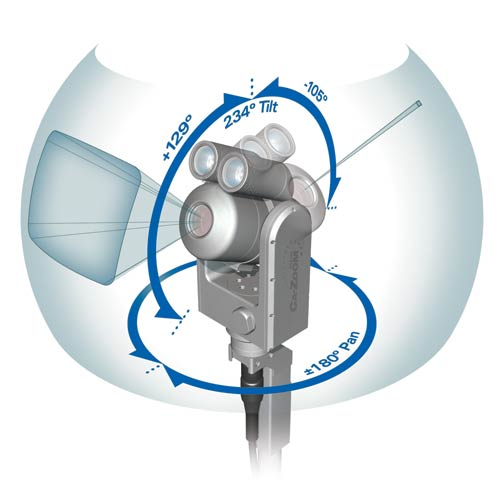
\includegraphics[width=0.6\linewidth]{mech_pantilt}
	\caption{PTZ kamera}
	\label{fig:mech_pantilt}
\end{figure}

A \ref{sec:valos}. bekezdésben vizsgált rendszerek is hasonlóképpen mozognak. Ezek közelebbi vizsgálata után elkezdtem kidolgozni a saját koncepciómat. Szemléltetésképpen készítettem a \ref{fig:megval_mockup}. ábrát. Az egyszerűség kedvéért a fegyver csövét egy síkba terveztem a pan és tilt tengelyekkel, ez megkönnyíti a későbbi számításokat.

\begin{figure}[h!]
	\centering
	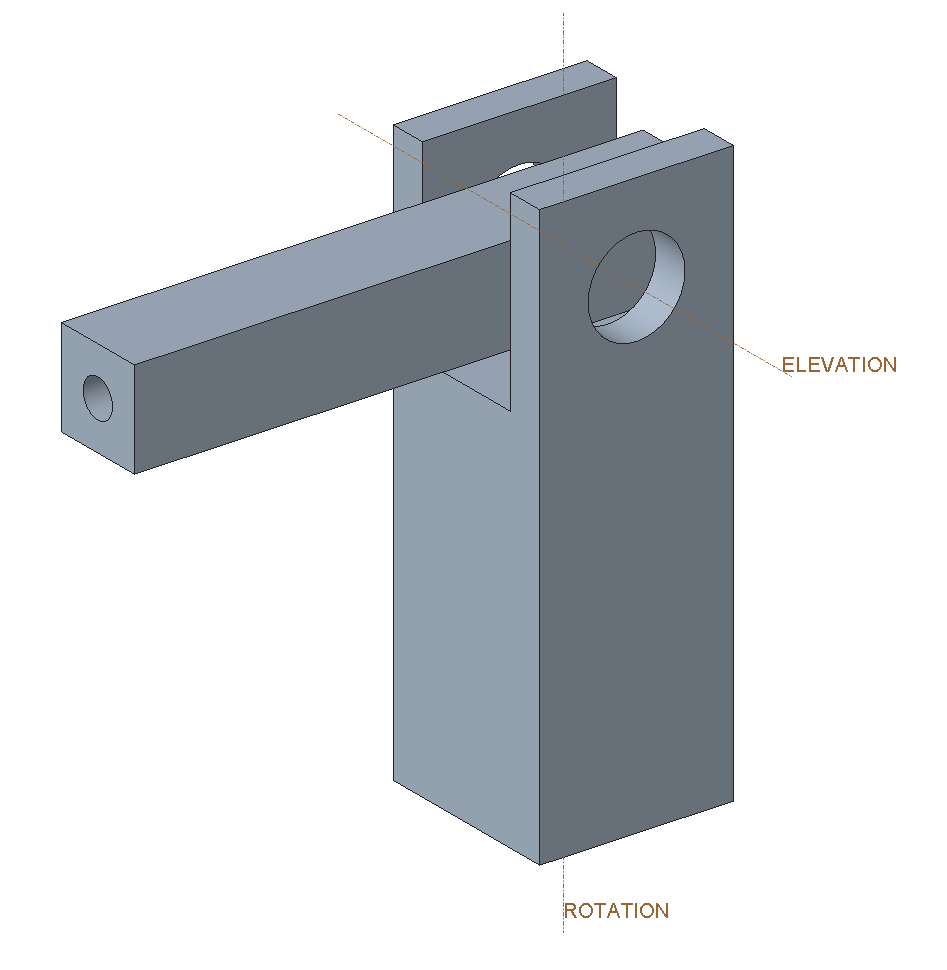
\includegraphics[width=0.6\linewidth]{mockup}
	\caption{Egyszerűsített kinematikai ábra}
	\label{fig:megval_mockup}
\end{figure}

Ki kellett számolnom bizonyos geometriai megkötéseket, amelyek szükségesek a tervezéshez, illetve az alkatrészek kiválasztásához. \\

A torony szükséges fordulatszámát a következőképpen lehet kiszámolni:


\begin{equation}
	rpm_{min} = \frac{v_t}{2 \cdot \pi \cdot r} = \frac{2.778 \w{m/s}}{2 \cdot \pi \cdot \w{m}} = 0.442 \w{1/s} = 26.526 \w{1/min}
\end{equation}

ahol:

\begin{tabular}{cl}
	$v_t$ & A célpont sebessége a fegyvercsőre merőlegesen, \\
	$r$ & A távolság a célpont és a rendszer között\\
\end{tabular}

Meg lehet állapítani a torony mozgásának felbontását is, tehát hogy hány fokonként lehet állítani a mozgását.

\begin{equation}
	\alpha_{min} = \arcsin\left(\frac{a}{2 \cdot r}\right) \cdot 2 = \arcsin\left(\frac{0.3 \w{m}}{2 \cdot 10 \w{m}}\right) \cdot 2 = 1.719 {^\circ}
\end{equation}

ahol:

\begin{tabular}{cl}
	$a$ & A célpont mérete  \\
	$r$ & A távolság a célpont és a rendszer között\\
\end{tabular}
\pagebreak
\section{Mechanikai alkatrészek}
\subsubsection*{Elsütő mechanizmus}
Az elsütő mechanizmusnak egy \textsl{Specna Arms M4}-ből kiszerelt gearbox-ot, illetve annak csövét és hop-up kamráját használtam. A gearbox működése során egy villanymotor több áttételen keresztül hátrahúz egy dugattyút, és azzal együtt a mögötte lévő rugót. Mindeközben a hop-up kamrában betöltődik egy golyó, és megáll a csőben. Ahogy a részlegesen fogazott fogaskerék elengedi a dugattyút, azt a rugó előrelöki, ezáltal a dugattyúkamrában nagy légnyomás keletkezik, ami a fegyver csövén keresztül tud kiegyenlítődni. Folyamatos működés során a motor egymás után húzza fel és engedi el a dugattyút, így amíg van golyó a tárban képes tüzelni. A gearbox belső alkatrészei a \ref{fig:mech_gearboxdiagram}. ábrán láthatóak. 

\begin{figure}[h!]
	\centering
	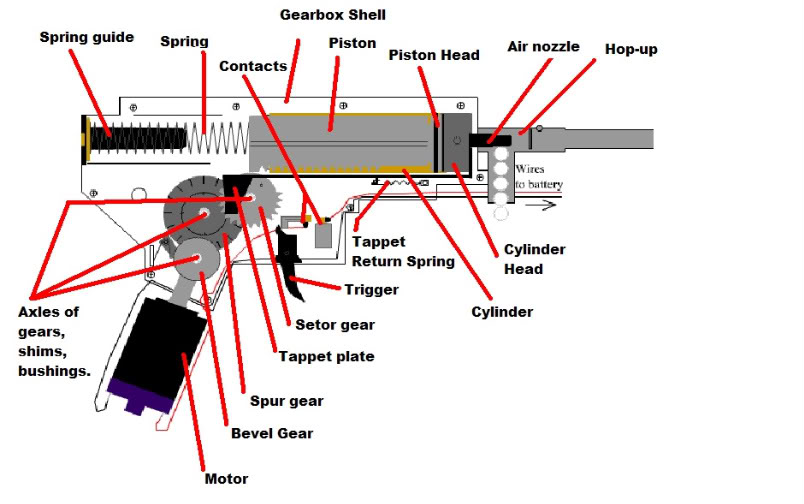
\includegraphics[width=1\linewidth]{mech_gearboxdiagram}
	\caption{V2 gearbox alkatrészei \cite{airsoft}}
	\label{fig:mech_gearboxdiagram}
\end{figure}

A hop-up kamrán belül még található egy gumi csúszófelület, amivel a kilőtt golyó perdületét lehet állítani, ezáltal pedig a fegyver effektív távolságát növelni.\\

A gearbox-on belül alakítanom kellett a működésen, hogy az előbb leírt folyamatos működést biztosítani tudjam.  Az elsütőbillentyűt, a tűzkapcsolót és minden ehhez tartozó mechanikai elemet kiszereltem, illetve áthuzaloztam. Erre azért volt szükség, mert különben csak a ravasz meghúzásával lehetett volna tüzelni, ami bonyolít a rendszer megvalósításán. A gearbox belső kialakítása a \ref{fig:gearboxbele}. ábrán látható. \\

\begin{figure}[h!]
	\centering
	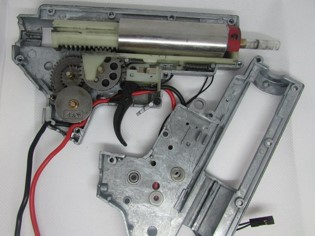
\includegraphics[width=0.6\linewidth]{gearboxbele}
	\caption{A gearbox belseje\cite{airsoft}}
	\label{fig:gearboxbele}
\end{figure}

A fegyver gearbox-ot körülvevő alkatrészeiről le tudtam venni méreteket, ez alapján alakítottam ki később a 3D nyomtatott alkatrészeket. Így végeredményben egy magába zárt alkatrészem lett, amin habár mechanikus nem lehet állítani a tüzelés módját, de csupán két vezetékkel csatlakozik az elektronikához. \\

A gearbox áramfogyasztását illetően találtam méréseket az interneten, ahol kifejezetten az én modellemet tesztelték. Az itteni mérések alapján arra következtettem, hogy 15 A-ra méretezni az áramkört megfelelő lehet. \cite{airsoftteszt}

\subsubsection*{Motorok}

A projekthez kettő \textbf{NEMA-17} léptetőmotort használok\cite{nema17}. Ezek a léptetőmotoroknak egy széles körben alkalmazott típusa, amelyeket főként precíziós mozgatási feladatokhoz használnak, például CNC gépekben, 3D nyomtatókban, robotikai alkalmazásokban és automatizálási rendszerekben. A NEMA-17 esetében a szám a motor elülső oldalának névleges méretét jelenti, amely 1.7 hüvelyk, azaz körülbelül 42,3 mm. \\

 A léptetőmotorok a mozgásukat apró, egyenlő lépésekre osztják, így lehetővé téve a precíz pozícionálást és sebességszabályozást. A NEMA-17 léptetőmotor tipikusan kétfázisú bipoláris motor, amely négy vezetékes tekercseléssel rendelkezik. Minden lépés során a motor egy adott szöggel fordul el, ami az adott motor típusától és felépítésétől függően tipikusan 1.8 fok, így teljes fordulat esetén 200 lépésre van szükség.\\

Az én esetemben használt léptetőmotorok lépésszöge 1.8 fok, bár ezt a motorvezérlőn lehet tovább osztani. A tartónyomatéka 0.4 Nm. Ezek a paraméterek 10-es áttételű fogaskerék-kapcsolattal megfelelőnek kell lenniük egy ilyen kis teljesítményű alkalmazásnál.

\pagebreak

\section{3D tervezés, modellezés}
A 3D tervezést Top-Down módszerrel végeztem, ez azt jelenti, hogy először az összeállítás szintjéről kezdem a tervezést, és egy úgynevezett skeleton modellbe veszem fel az egyes alkatrészek méreteit. Ezáltal tudom garantálni az egymáshoz való illeszkedést, valamint a változtatások könnyű implementálását.\\

\subsection{Skeleton modell}
A modellezést a skeleton modellek megalkotásával kezdtem. A fő összeállításon belül két skeleton modellt hoztam létre, mivel maga a modell két alösszeállítása jól elkülöníthető egymástól.

\begin{figure}[h!]
	\centering
	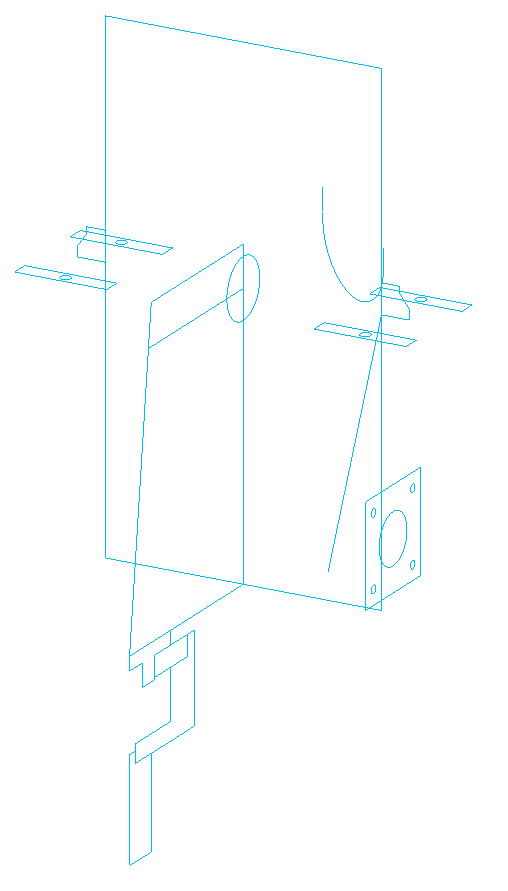
\includegraphics[width=0.5\linewidth]{mech_skeleton1}
	\caption{DT-9999 skeleton modell}
	\label{fig:mech_skeleton1}
\end{figure}

Az egyik (\ref{fig:mech_skeleton1}.ábra) alkatrészei rendszerint a függőleges tengely körül szimmetrikusak, a másiké (\ref{fig:mech_skeleton2}.ábra) pedig a fegyver csöve körül.

\begin{figure}[h!]
	\centering
	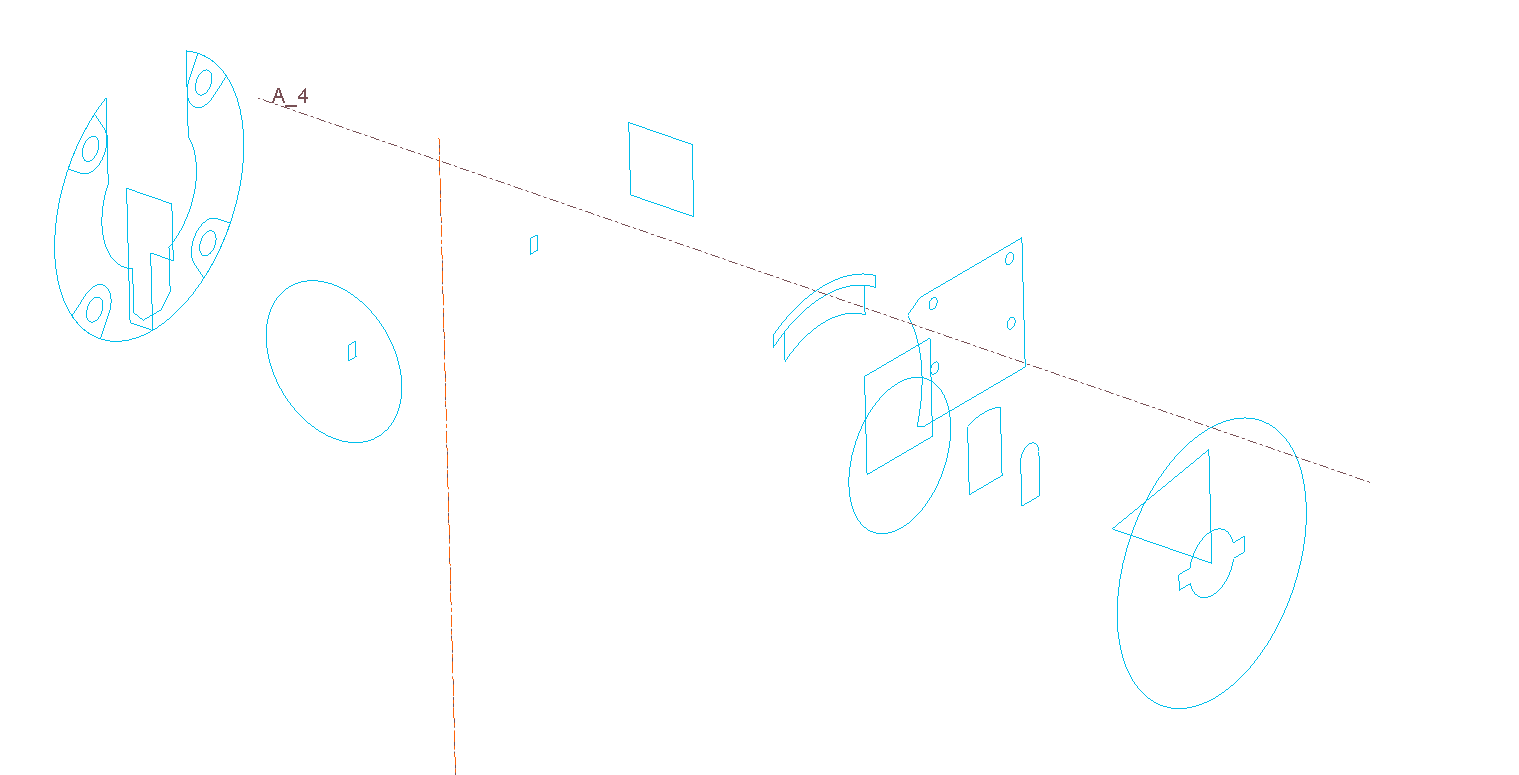
\includegraphics[width=1\linewidth]{mech_skeleton2}
	\caption{DT-4999 skeleton modell}
	\label{fig:mech_skeleton2}
\end{figure}

Az ábrákon láthatóak a vázlatok és tengelyek, amelyek alapján kialakítottam az egyes alkatrészeket. Sok méretet először csak hozzávetőlegesen vettem fel, pl. a torony magasságát. A Top-Down módszer előnye, hogy később ezeket könnyedén módosíthatom, és az alkatrészek frissítés után ugyanúgy fognak egymáshoz illeszkedni.


\subsection{Torony}

Elsőként a \textbf{gearbox tartó elemet} kezdtem el tervezni, mert maga a gearbox volt a tervezés elején az egyetlen elem, amiből tudtam következtetni a szükséges méretekre. Erről kép a \ref{fig:mech_dt4000}. ábrán látható. 

\begin{figure}[h!]
	\centering
	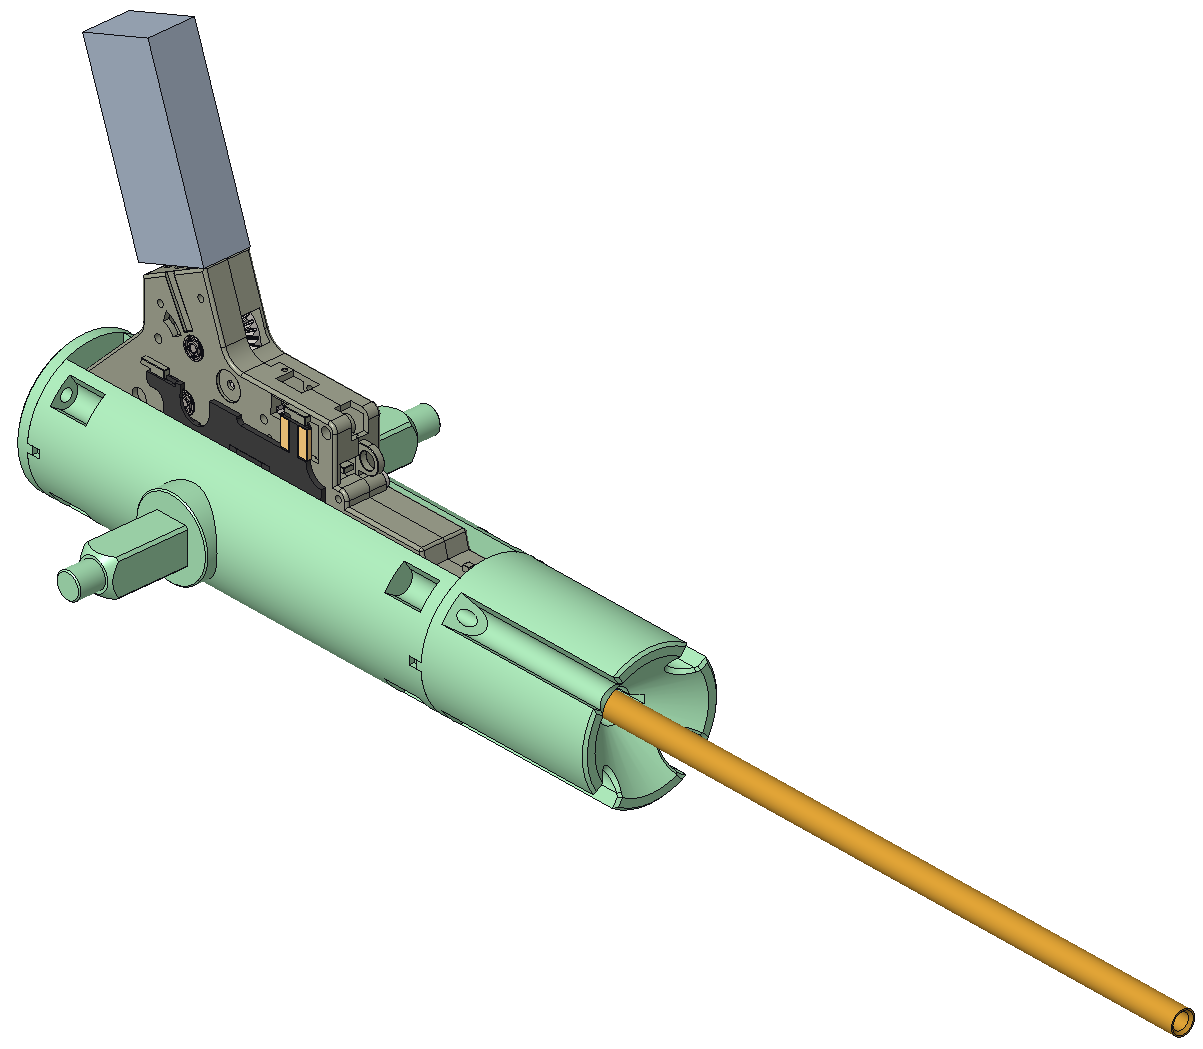
\includegraphics[width=0.8\linewidth]{mech_dt4000}
	\caption{Gearbox tartó ház}
	\label{fig:mech_dt4000}
\end{figure}

A gearbox ház 3 alkatrészből áll, egy központi elemből, valamint két fedélből a végein. A kialakítást a teljes airsoft fegyver alapján terveztem, hogy ugyanúgy álljon a gearbox mint az eredeti felhasználása során. A kritikusabb rész ebben az elemben a hop-up kamra körüli kialakítás volt, itt elég komplex volt a geometria, de a 3D nyomtatás lehetővé tette a megvalósítást. Ezt a \ref{fig:mech_dt4200}. ábrán lehet látni.


\begin{figure}[h!]
	\centering
	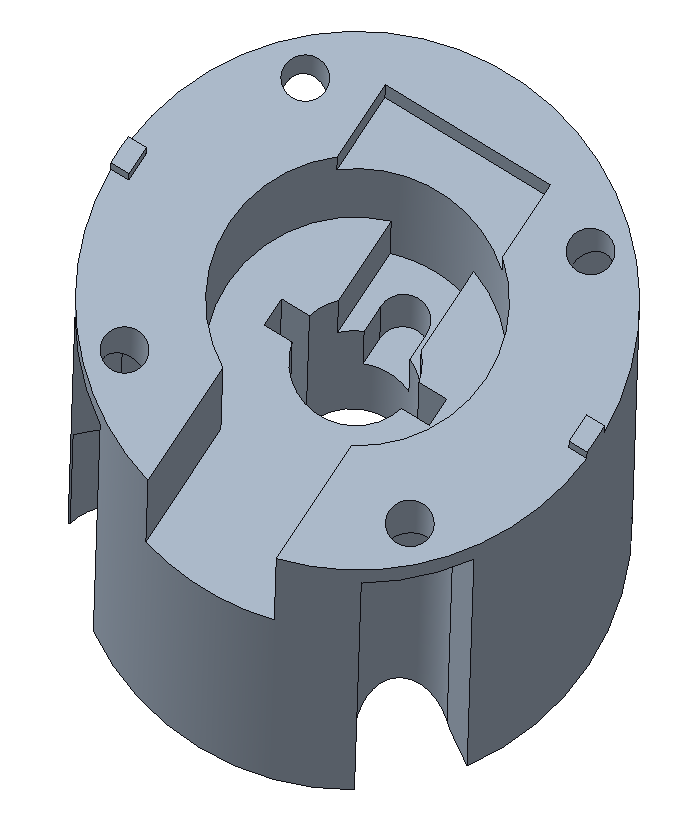
\includegraphics[width=0.4\linewidth]{mech_dt4200}
	\caption{Hop-Up kamra körüli elem}
	\label{fig:mech_dt4200}
\end{figure}


A következő alösszeállítás a \textbf{tár} volt, amely a gearbox ház bal oldali tengelyére csatlakozik. Ennek kialakítása a \ref{fig:mech_tar}. ábrán látható. A 6 mm-es golyók a zöld kupak nyílásán keresztül tölthetőek a lila tárba. Alul és felül 1-1 gumigyűrű feszíti előre a zöld dugattyút, ami a tár kúpos végén keresztül nyomja ki a golyókat. Így mechanikailag, plusz elektronika nélkül biztosítható a fegyver lövedékkel való ellátása, és szemmel is látható a tár töltöttségi szintje.

\begin{figure}[h!]
	\centering
	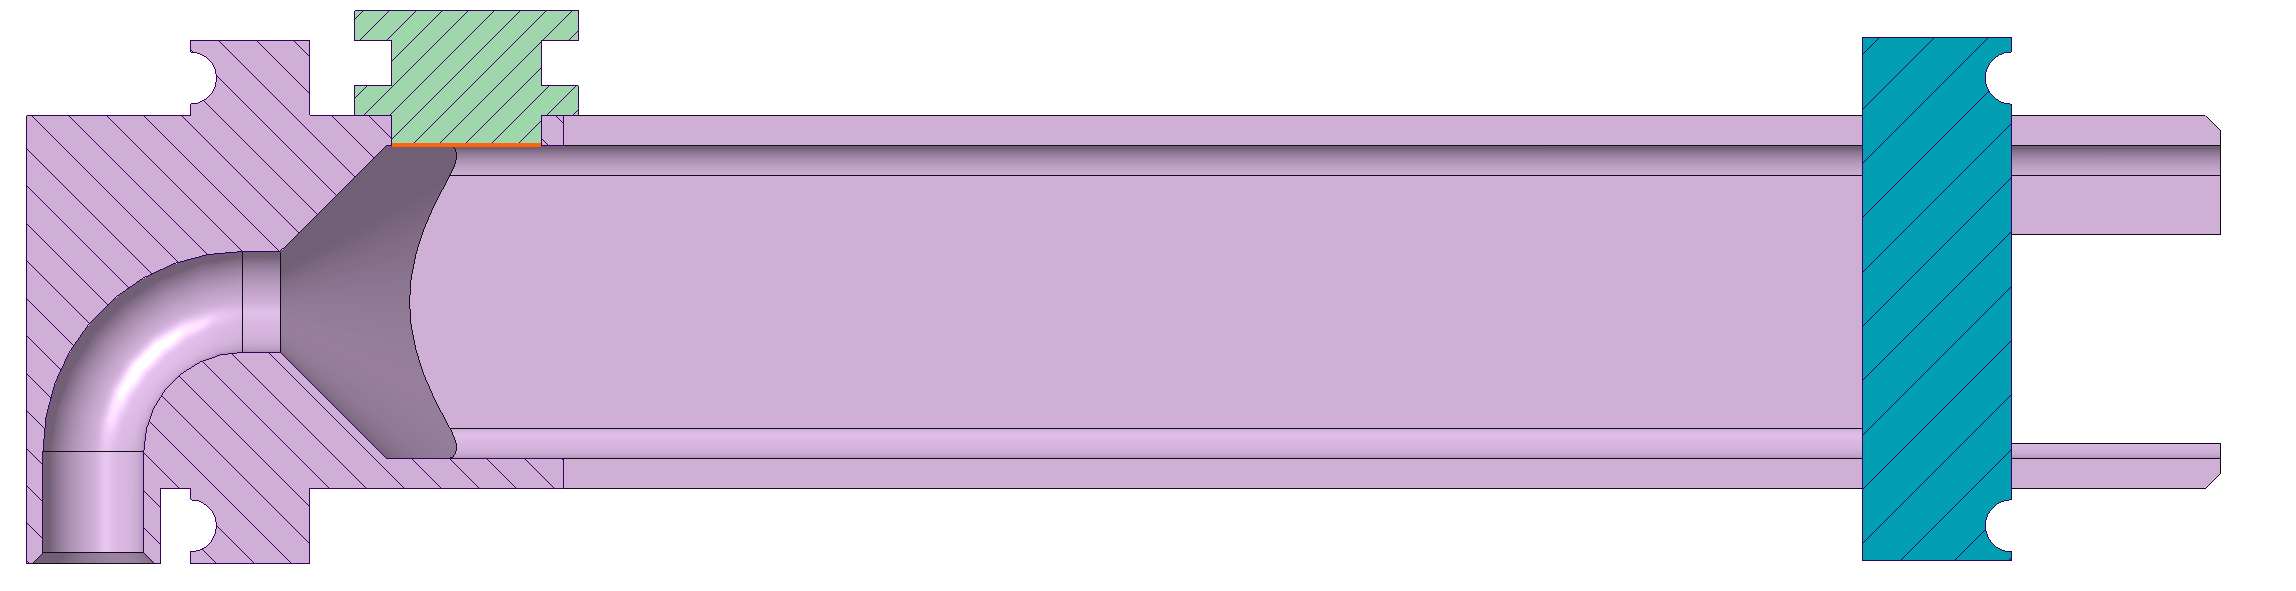
\includegraphics[width=1\linewidth]{mech_tar}
	\caption{Tár}
	\label{fig:mech_tar}
\end{figure}

Ez a kialakítás végül nem volt sikeres, ugyanis a golyók nagyon könnyedén elakadtak, gyakorlatilag egyszer sem sikerült lőni vele. Újragondolás után egy hasonló megoldást használtam, ám a golyók egyesével sorakoznak a tárban, ez látható a \ref{fig:mech_tar2}. ábrán.



\begin{figure}[h!]
	\centering
	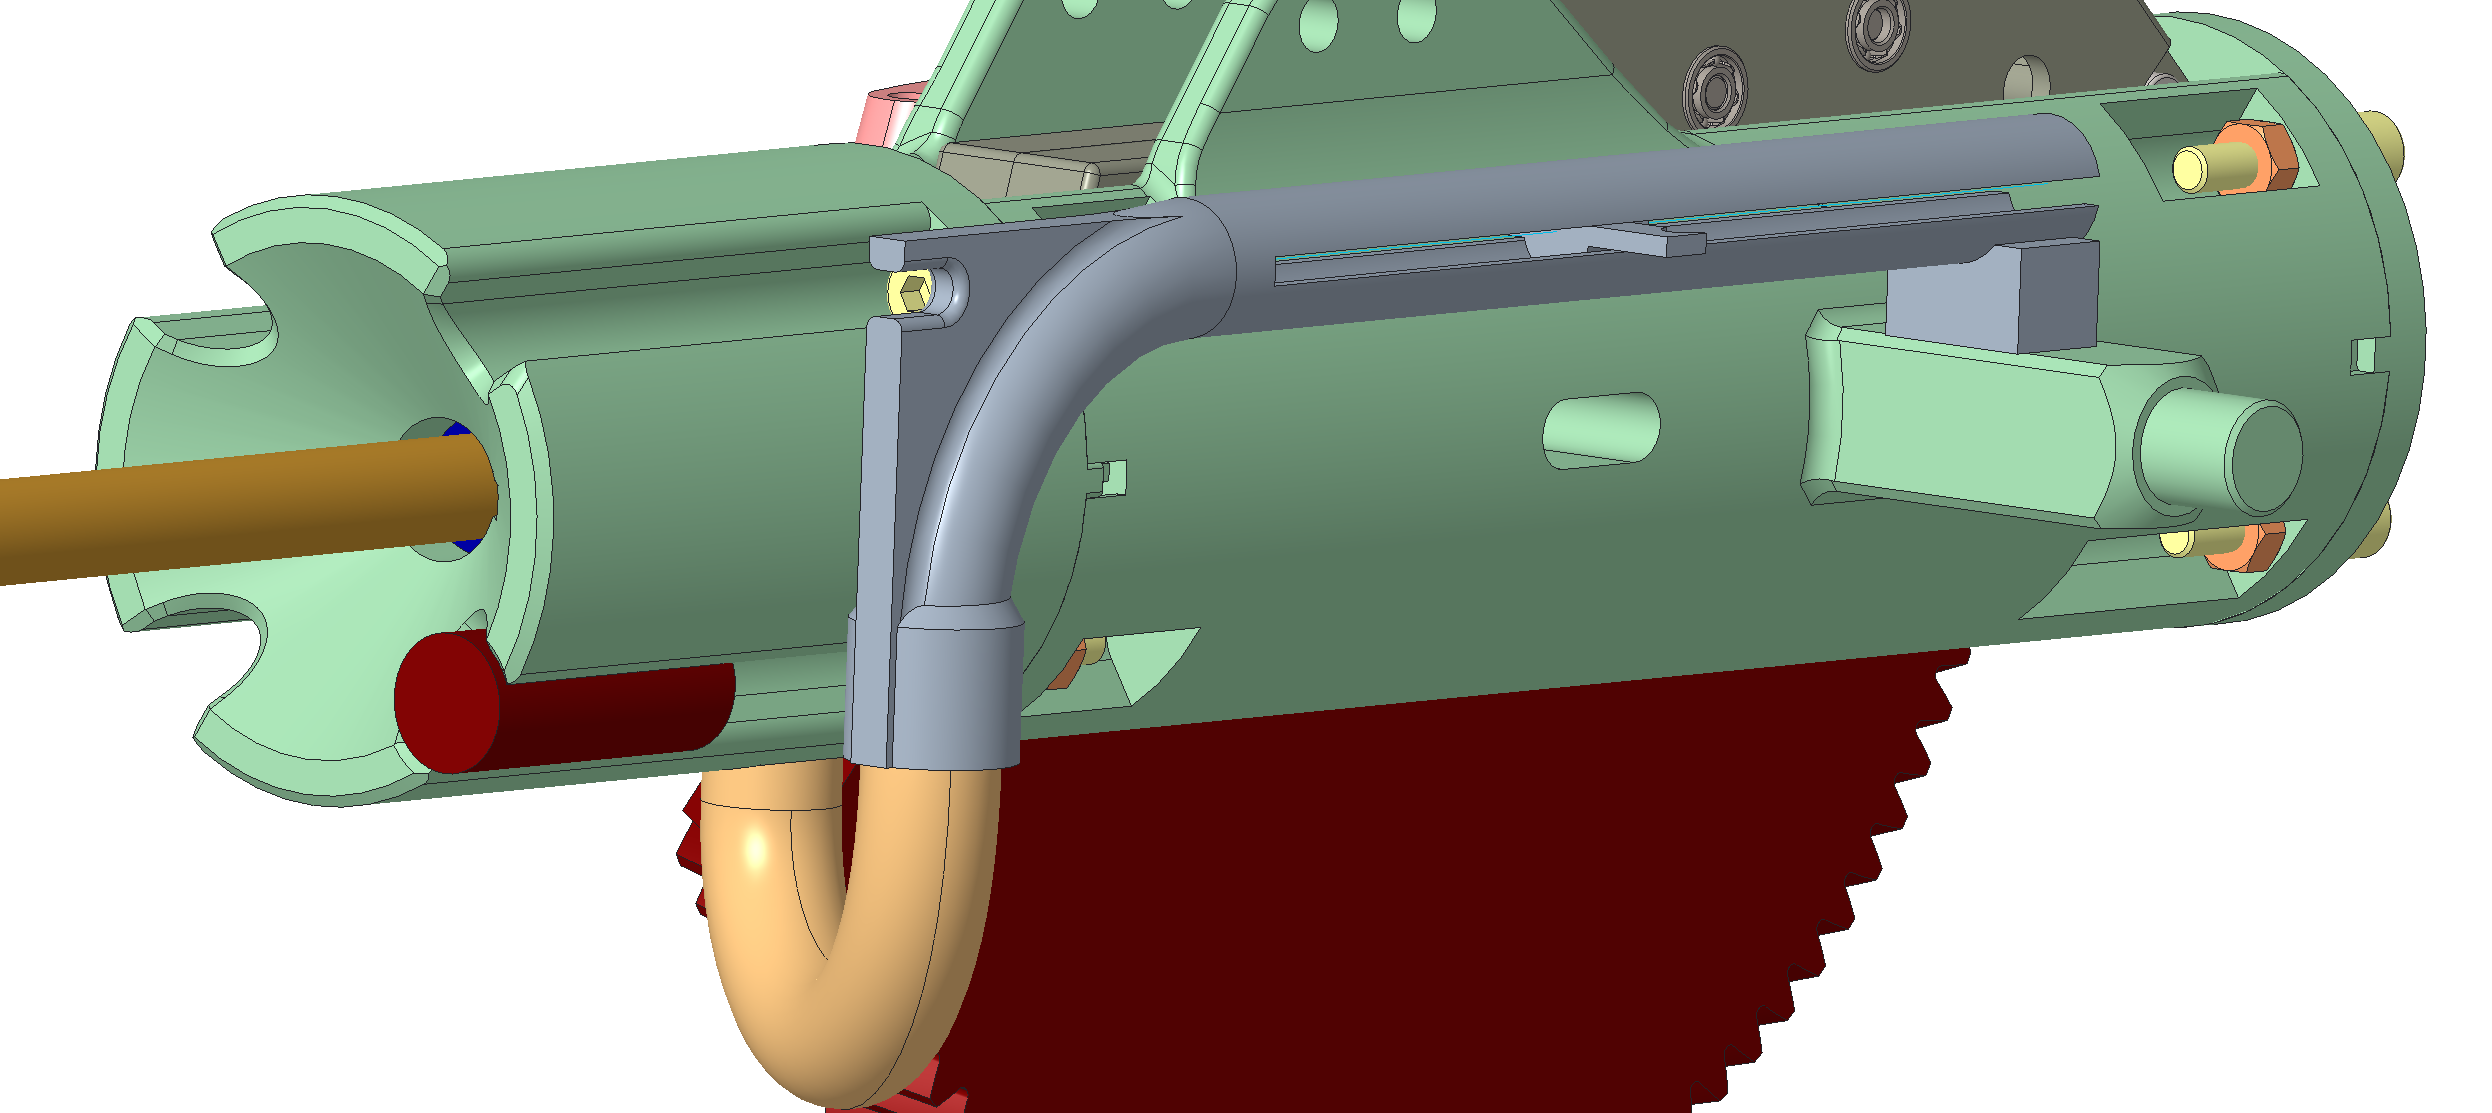
\includegraphics[width=1\linewidth]{mech_tar2}
	\caption{Új tár}
	\label{fig:mech_tar2}
\end{figure}
Végül a toronyra kerültek az elektronikai alkatrészek is, ezek a \ref{fig:mech_dt4000kamera}. ábrán láthatóak. A lila elem a lézer modul, a piros pedig a kamera konzol. Mind a kettő ragasztással kerül rögzítésre. Fontosnak tartottam, hogy ezek az elemek közvetlenül ahhoz az elemhez legyenek rögzítve, ami a fegyver csövét is pozicionálja, azonban a kamera esetén a 3D nyomtathatóság miatt egy konzolt szükségesnek éreztem.

\begin{figure}[h!]
	\centering
	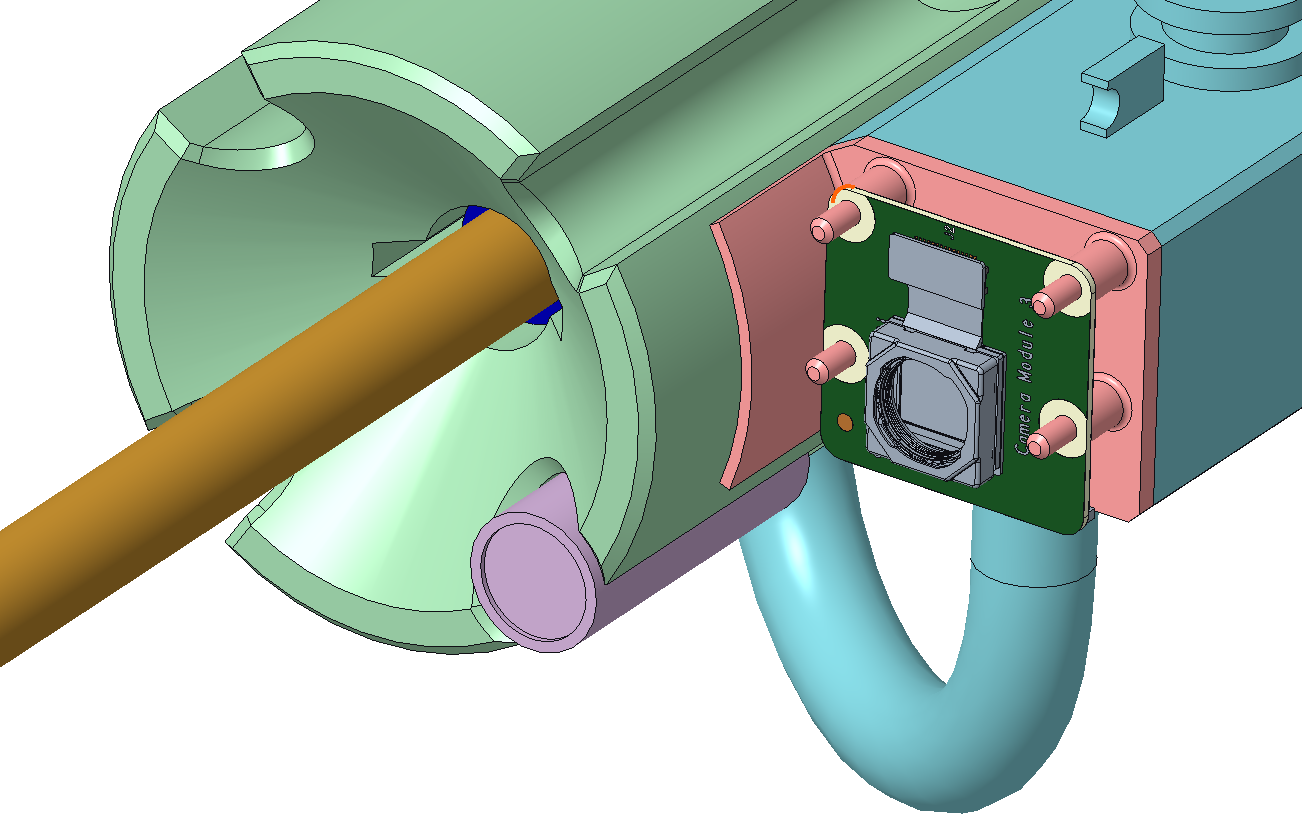
\includegraphics[width=1\linewidth]{mech_dt4000kamera}
	\caption{Kamera és lézer modul beépítés}
	\label{fig:mech_dt4000kamera}
\end{figure}

\subsection{Keret}
Az úgynevezett \textbf{keret} volt a konstrukció legösszetettebb eleme, és egyben a legnagyobb térfogatú is. Fő funkciója a torony stabil tartása a csapágyakkal együtt. Ezentúl erre az elemre van rögzítve a vezérlőelektronika nagy része, a végálláskapcsolók és a vízszintes tengelyhez tartozó motor is. Ez az elem az alatta lévő alkatrészhez ragasztással lett rögzítve, hogy a szerelést egyszerűsítsem. A csapágyak támasztása X elrendezésű, és az osztott "csapágyház" miatt könnyen szerelhetőek. A csapágy elrendezése a \ref{fig:mech_felsotengely}. ábrán látható.

\begin{figure}[h!]
	\centering
	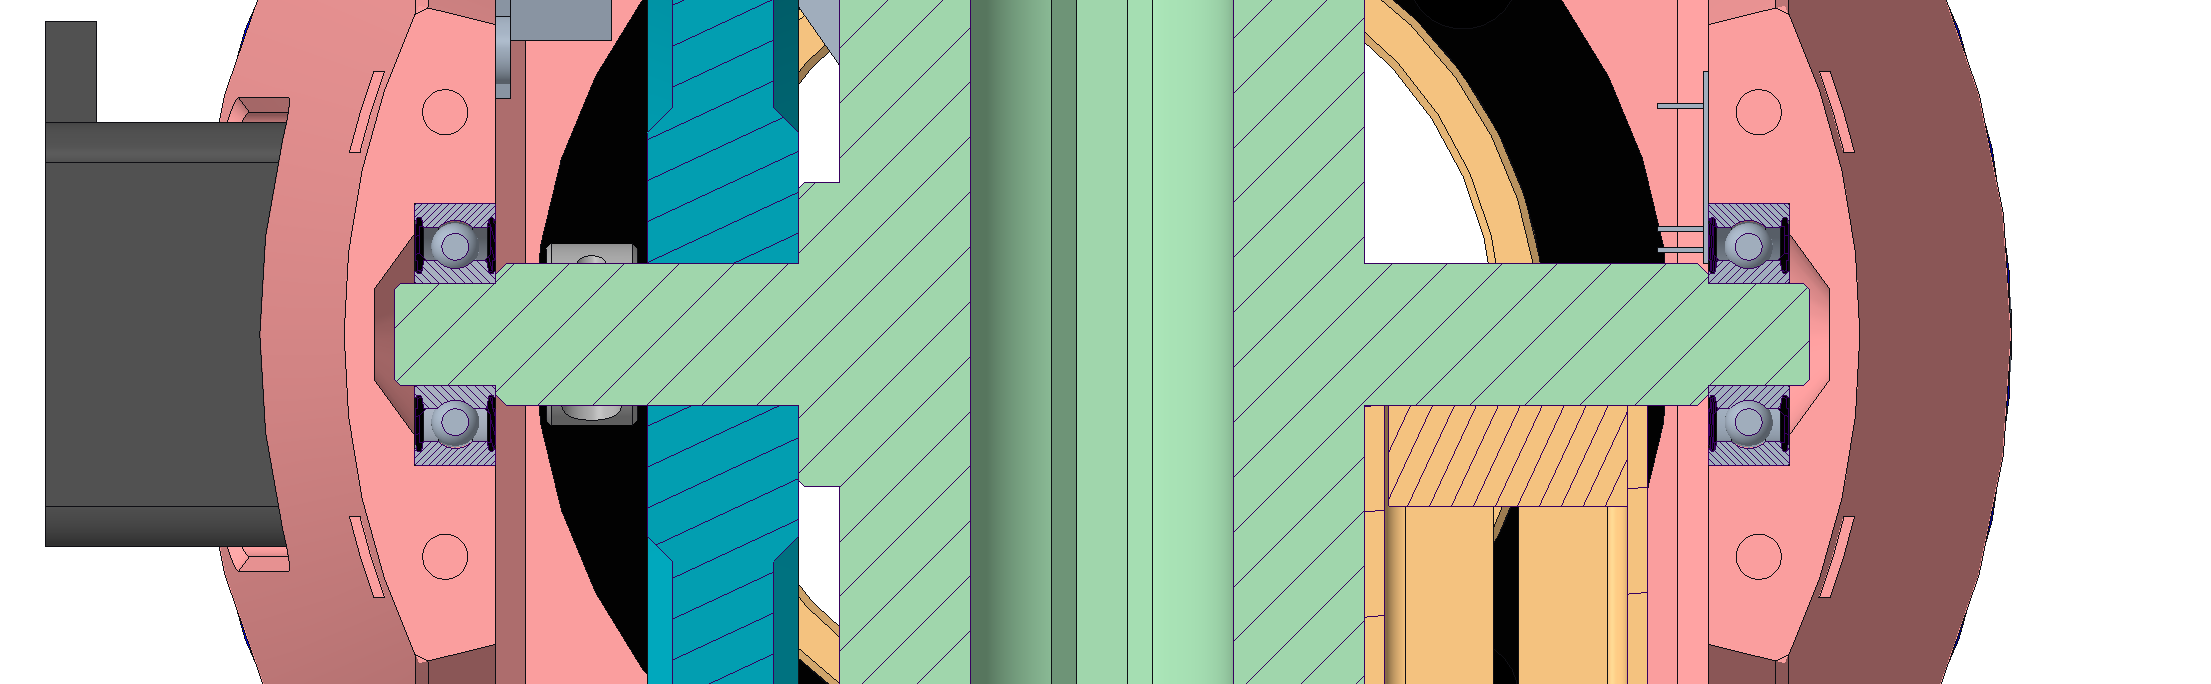
\includegraphics[width=1\linewidth]{mech_felsotengely}
	\caption{Vízszintes tengely csapágyainak elrendezése}
	\label{fig:mech_felsotengely}
\end{figure}


Kétséges rész volt a \textbf{motor} rögzítése, ugyanis nagy szükség van a pontos illeszkedésre. A nyomtatás irányára azonban a motor központosítására szánt furat pont merőleges, de szerencsére a nyomtató így is elég nagy pontosságot tudott elérni.

\begin{figure}[h!]
	\centering
	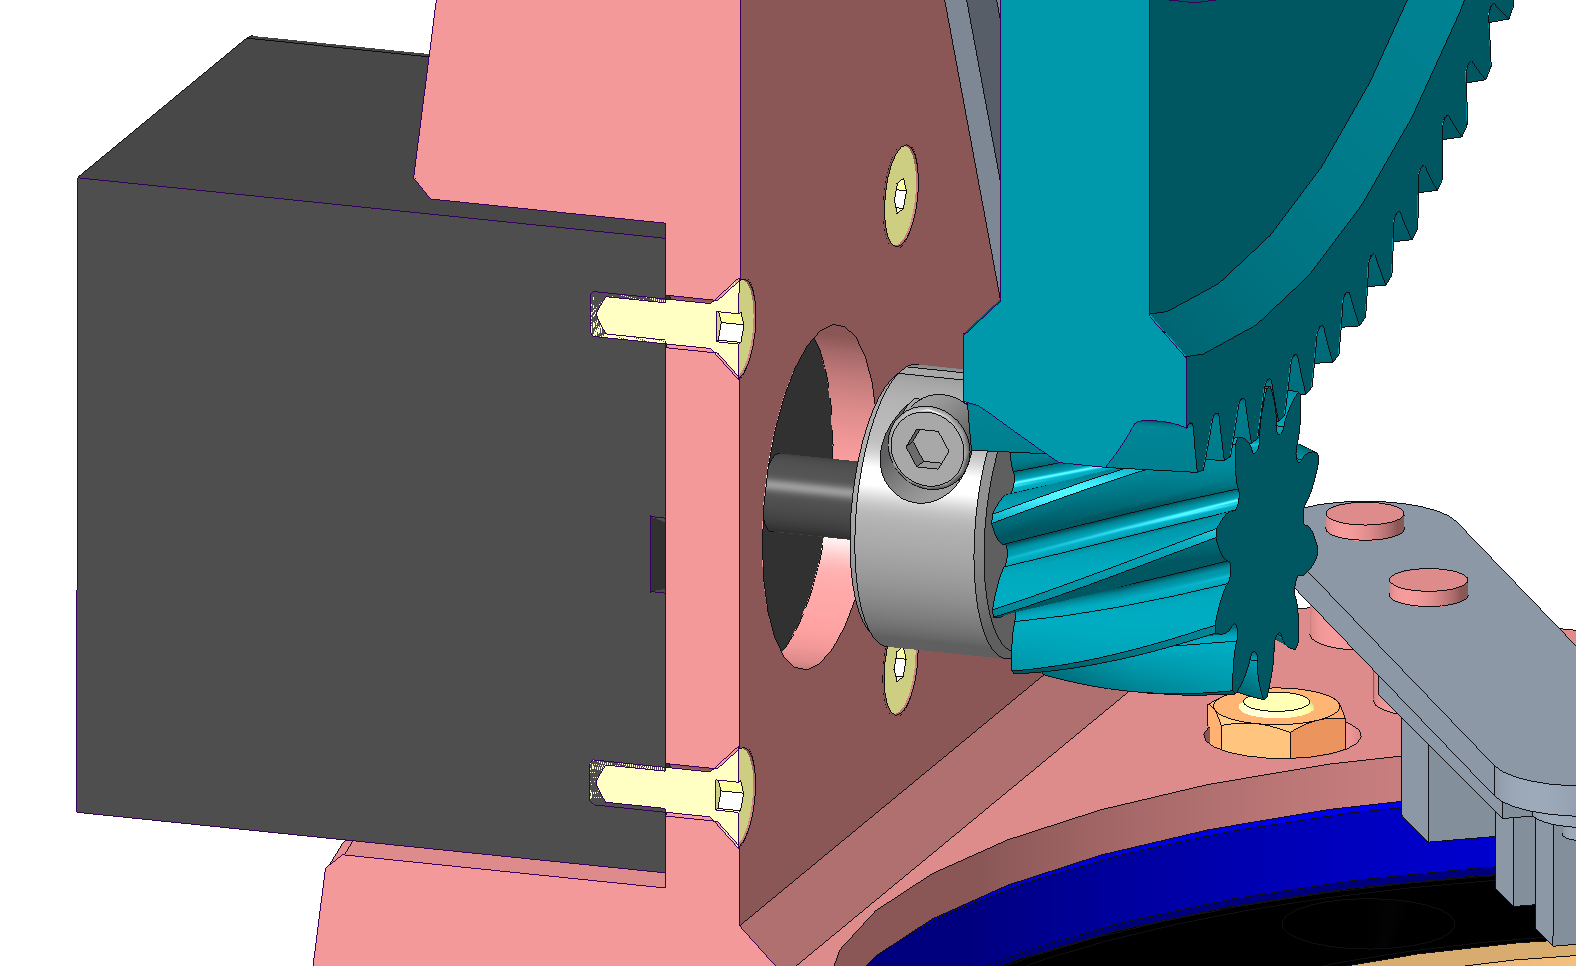
\includegraphics[width=1 \linewidth]{mech_motorbeepites}
	\caption{Vízszintes tengely motor beépítése}
	\label{fig:mech_motorbeepites}
\end{figure}

A kereten kaptak helyet a végálláskapcsolók is, amivel a rendszer indításkor kalibrálható. A egyik a vízszintes tengely nagy fogaskerekéhez, a másik pedig a függőleges tengely központi eleméhez viszonyít.


\begin{figure}
	\centering
	\begin{minipage}{.5\textwidth}
		\centering
		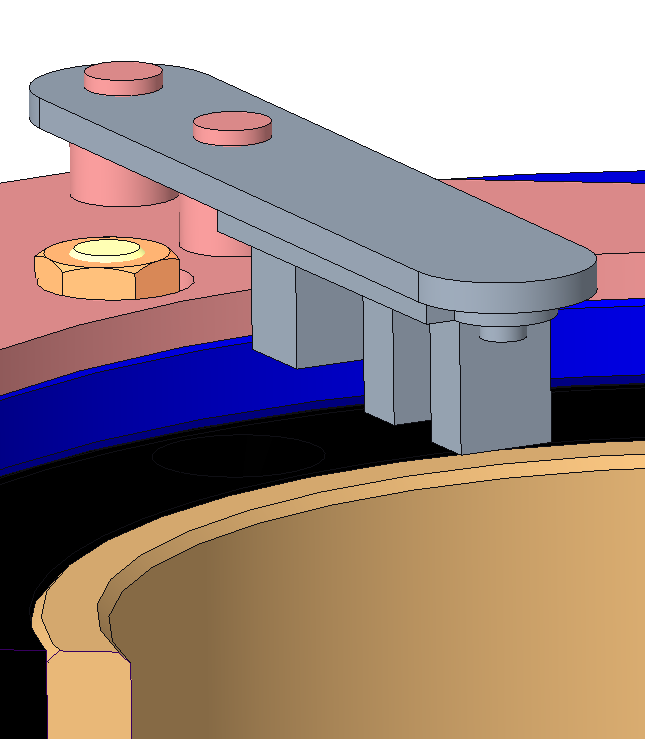
\includegraphics[width=.7\linewidth]{mech_vegallas1}
		\caption{Pan végálláskapcsoló}
		\label{fig:mech_vegallas1}
	\end{minipage}%
	\begin{minipage}{.5\textwidth}
		\centering
		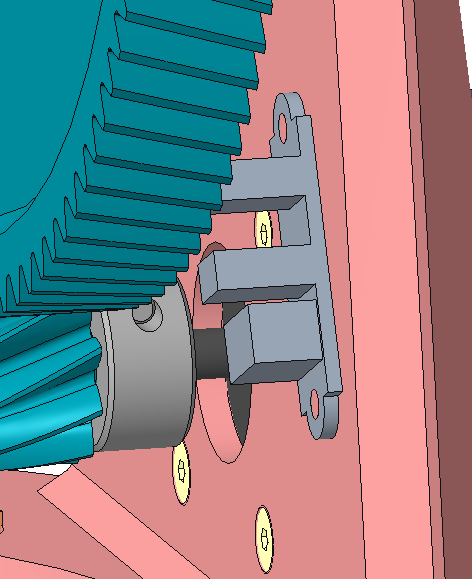
\includegraphics[width=.7\linewidth]{mech_vegallas2}
		\caption{Tilt végálláskapcsoló}
		\label{fig:mech_vegallas2}
	\end{minipage}
\end{figure}

\subsection{Függőleges tengely elemei}

Utolsó lépésként megterveztem a függőleges tengely mozgatásáért felelős elemeket. ezek kialakítása a \ref{fig:mech_alsoreszek}. ábrán látható. A narancssárga alakrész a központi elem, amelynek feladata a csapágy támasztása és a motor rögzítése. A motor vezetékei, valamint az elektronikából kilógó többi kábel ennek a közepén fut keresztül. A csapágy egyik fele ehhez az elemhez van rögzítve, a másik pedig  az ábrán kékkel ábrázolt alkatrészhez. Erre a kék elemre került rögzítésre a belsőfogazású fogaskerék is. \\ 

A sárga alkatrész a talapzat része. Ez a legnagyobb kiterjedésű elem az egész modellben. Hogy elkerüljem a támaszanyag használatát, a csavarok fejeinek felfekvő felületeit egy külön alkatrész ragasztásával oldottam meg. Ez a talp 45 fokos belső felületére illeszkedik, és ragasztással kerül rögzítésre. A 4 oldalán kialakításra kerültek csatlakozó felületek, ahol különböző lábak helyezhetők az eszközre.

\begin{figure}[h!]
	\centering
	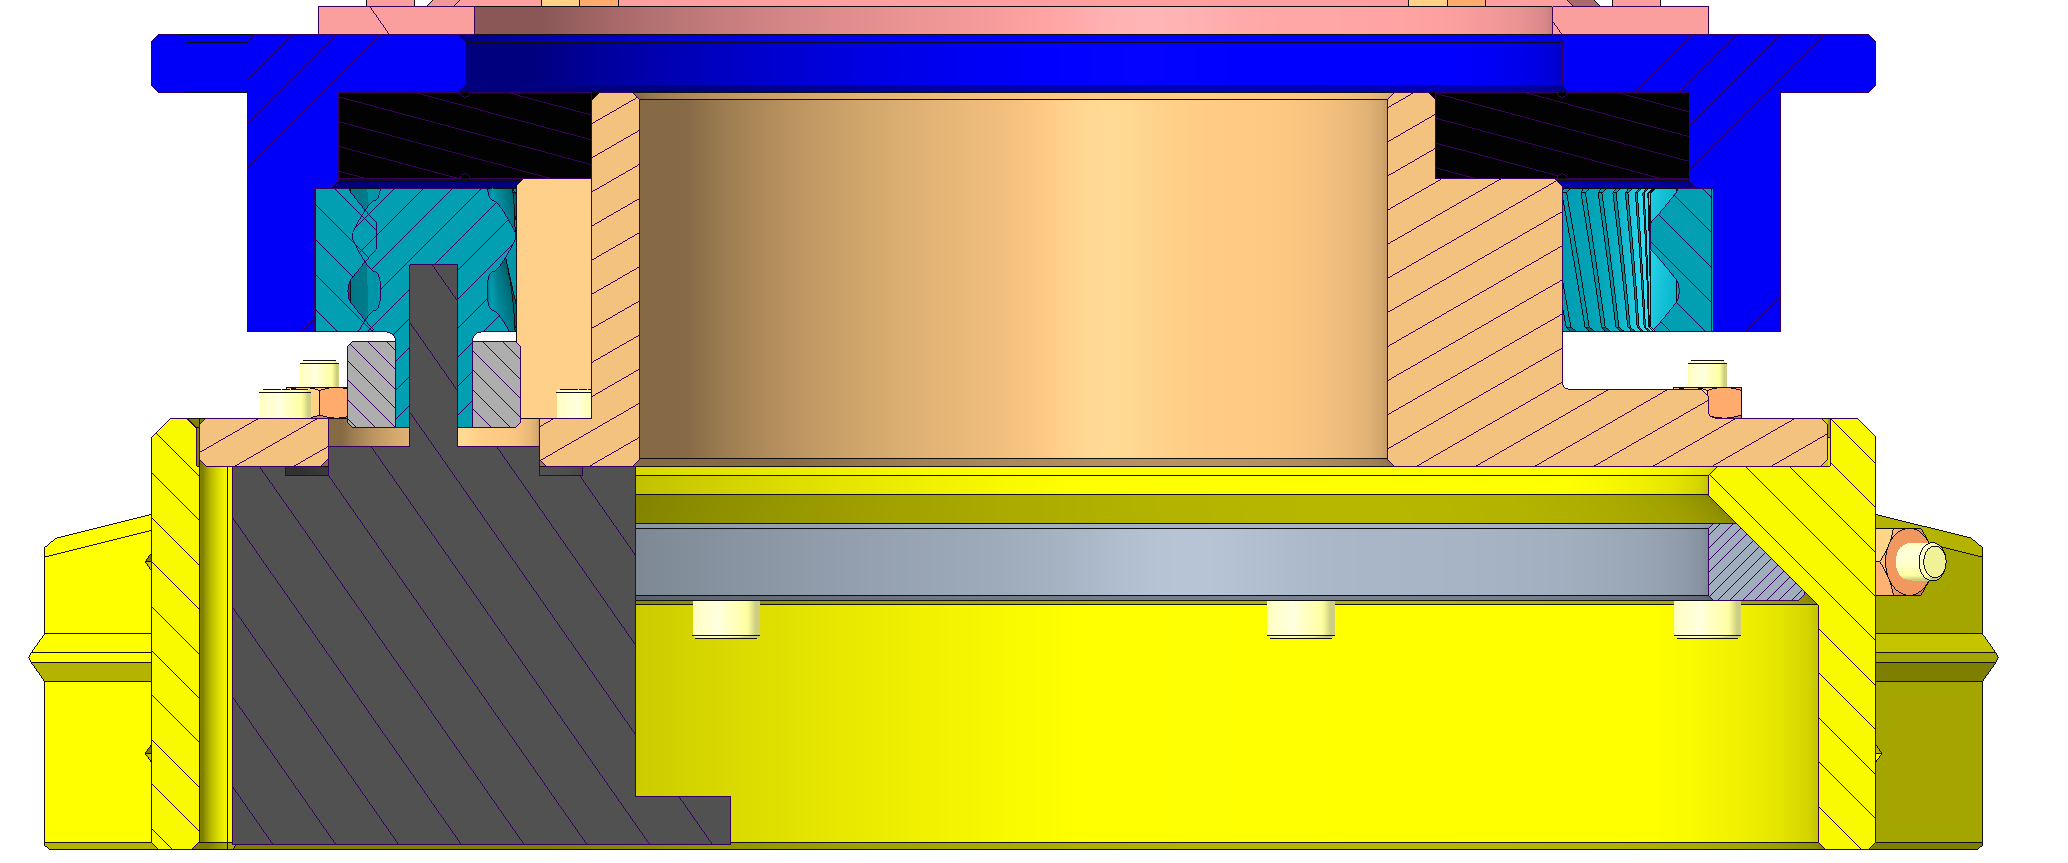
\includegraphics[width=1\linewidth]{mech_alsoreszek}
	\caption{Függőleges tengely elrendezése}
	\label{fig:mech_alsoreszek}
\end{figure}

\subsection{Fogaskerekek}
A prototípusban két fogaskerék kapcsolat kapott helyet. A függőleges tengely nagy fogaskereke belső fogazású, ezáltal el tudtam rejteni a motort a váz belsejében és kompaktabb lett a kialakítás, valamint valamivel stabilabb is. A kapcsolat áttétele 10, és ferde fogazású, ezáltal a futás csendesebb és egyenletesebb lett. A kapcsolat illusztrációja a \ref{fig:mech_fogpar1}. ábrán látható.

\begin{figure}[h!]
	\centering
	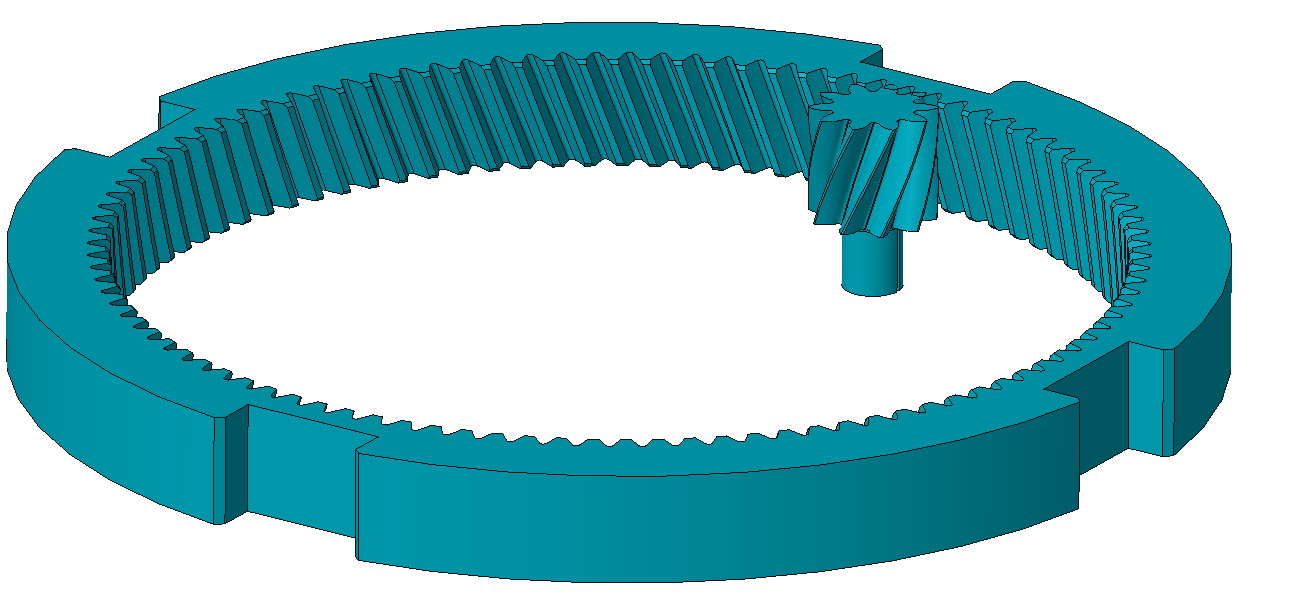
\includegraphics[width=1\linewidth]{mech_fogpar1}
	\caption{Függőleges tengely fogaskerekek}
	\label{fig:mech_fogpar1}
\end{figure}

A vízszintes tengely nagy fogaskereke a gearbox ház tengelyére lett erősítve, és csak részlegesen lett kinyomtatva. Ennek egyszerű oka, hogy más geometria is blokkolja a mozgást ezekben a tartományokban, illetve a Pan-Tilt kinematika mozgása redundáns lenne, ha teljesen körbe tudna forogni. A kapcsolat a \ref{fig:mech_fogpar1}. ábrán látható.

\begin{figure}[h!]
	\centering
	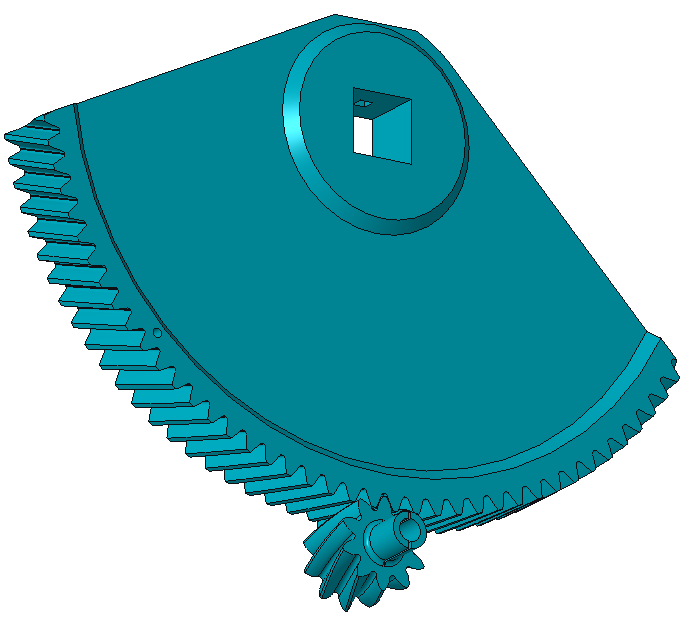
\includegraphics[width=0.5\linewidth]{mech_fogpar2}
	\caption{Vízszintes tengely fogaskerekek}
	\label{fig:mech_fogpar2}
\end{figure}

Mind a két fogaskerékpár kisebb tagja közvetlenül a motor tengelyére lett rögzítve, egy acél rögzítőgyűrűvel. Ennek kialakítása a \ref{fig:mech_alsoreszek}. ábra bal oldalán látható.

\pagebreak

\section{Gyártás és összeszerelés}
\subsection{Gyártás}



Minden egyedi alkatrészt, amit a projekthez kellett gyártanom, 3D nyomtatással készítettem el. Ehhez egy \textbf{Bambu Lab A1} \cite{bambu} típusú hobbinyomtatót használtam, amely a \ref{fig:mech_bambu}. ábrán látható. Mint a legtöbb ilyen árkategóriában lévő gép, ez is \textsl{FDM} technológiát használ. Az \textsl{FDM} lényege, hogy a nyomtató egy előre megadott terv alapján vékony műanyagszálat (filamentet) olvaszt meg egy forró extruderfejben (hotend), amelyet pontosan irányítanak a nyomtató XYZ tengelyei mentén. A műanyag szál olvasztott állapotban kerül a nyomtatóágyra, ahol gyorsan megszilárdul, így rétegenként építi fel az adott objektumot.\\

\begin{figure}[h!]
	\centering
	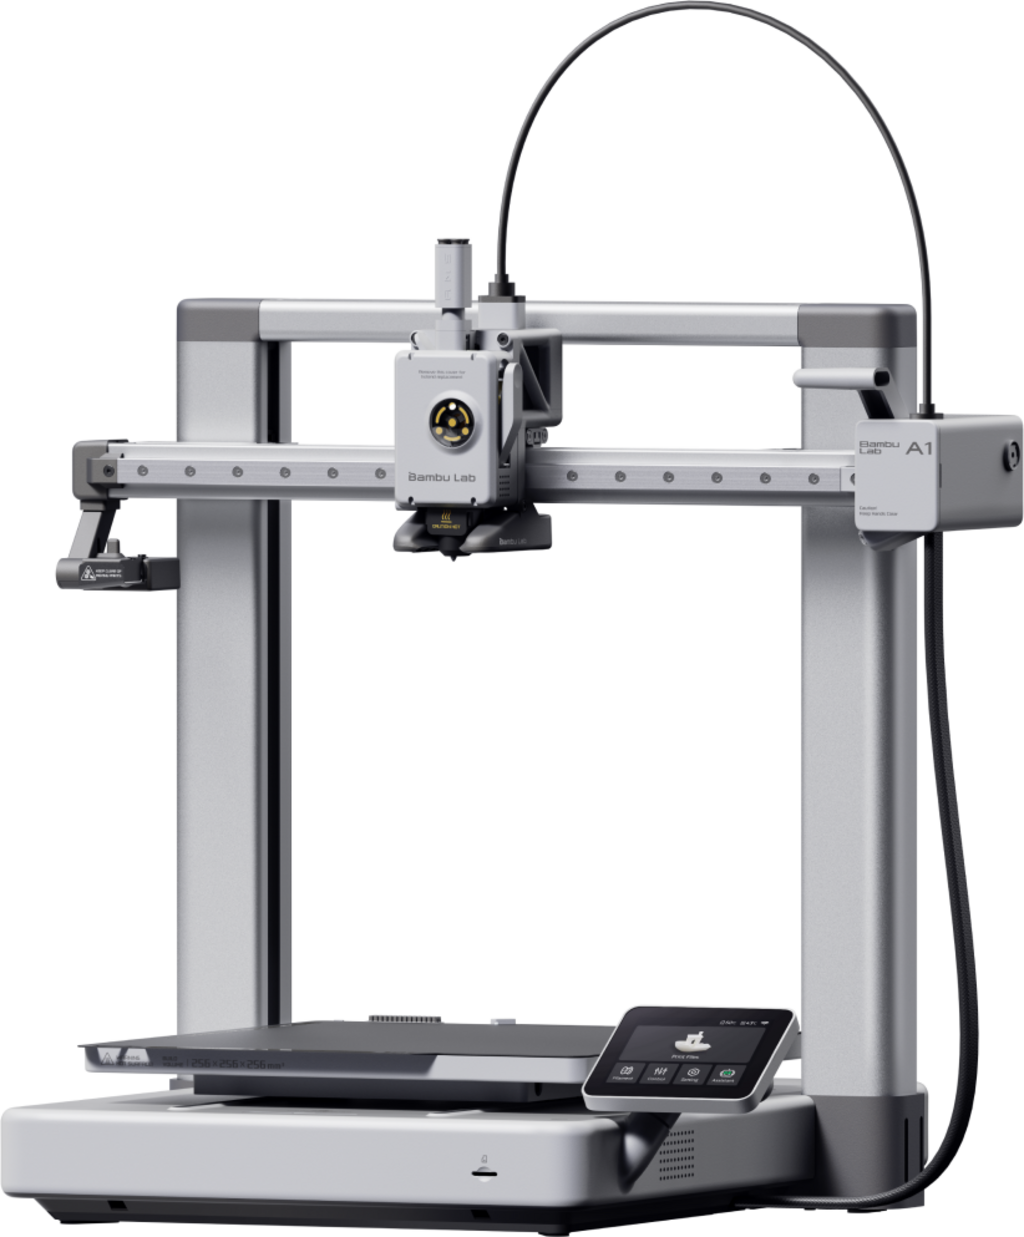
\includegraphics[width=.7\linewidth]{mech_bambu} 
	\caption{Bambu Lab A1}
	\label{fig:mech_bambu}
\end{figure}
\pagebreak

A használt nyomtató bizonyos tulajdonságai meghatározták a tervezett alkatrészek tulajdonságait:

\begin{itemize}
	\item \textbf{Nyomtatási térfogat:} 256 × 256 × 256 mm, amely elég nagy volt a legtöbb általam tervezett elem számára.
	\item \textbf{Nyomtatási pontosság:} A nyomtató rétegvastagsága 0,1–0,4 mm között állítható. Főleg a nyomtatott fogaskerekeknél volt fontos a megfelelő pontosság, de kielégítő eredmény született.
	\item \textbf{Használható filamentek:} A nyomtató különféle anyagokkal kompatibilis, beleértve a PLA-t, ABS-t, PETG-t és TPU-t. Én a PLA mellett döntöttem, ugyanis nem szükséges a pl. ABS által nyújtott minőség, ellenben a költséghatékonyság igen.
\end{itemize}

A modelleket \textbf{PTC Creo} szoftverben készítettem. Ez egy magas szintű CAD tervező program, amely képes a modelleket exportálni STEP és STL fájlként is. Az STL fájlokat ezután a Bambu Studio slicer programba betöltve tudtam a nyomtató által követhető G-kódra konvertálni. Itt kellett megtervezni a támasztást (\ref{fig:mech_bambustudio1}. ábra), illetve megadnia a nyomtatási paramétereket, amelyek a függelék \ref{sec:slicerbeallitasok}. fejezetében láthatóak. Ezután már csak meg kellett várni, amíg a gép elkészíti az adott alkatrészt, ami a legnagyobb elem esetén kb. 10 óra volt, a teljes prototípus kb. 50 óra volt.

\begin{figure}[h!]
	\centering
	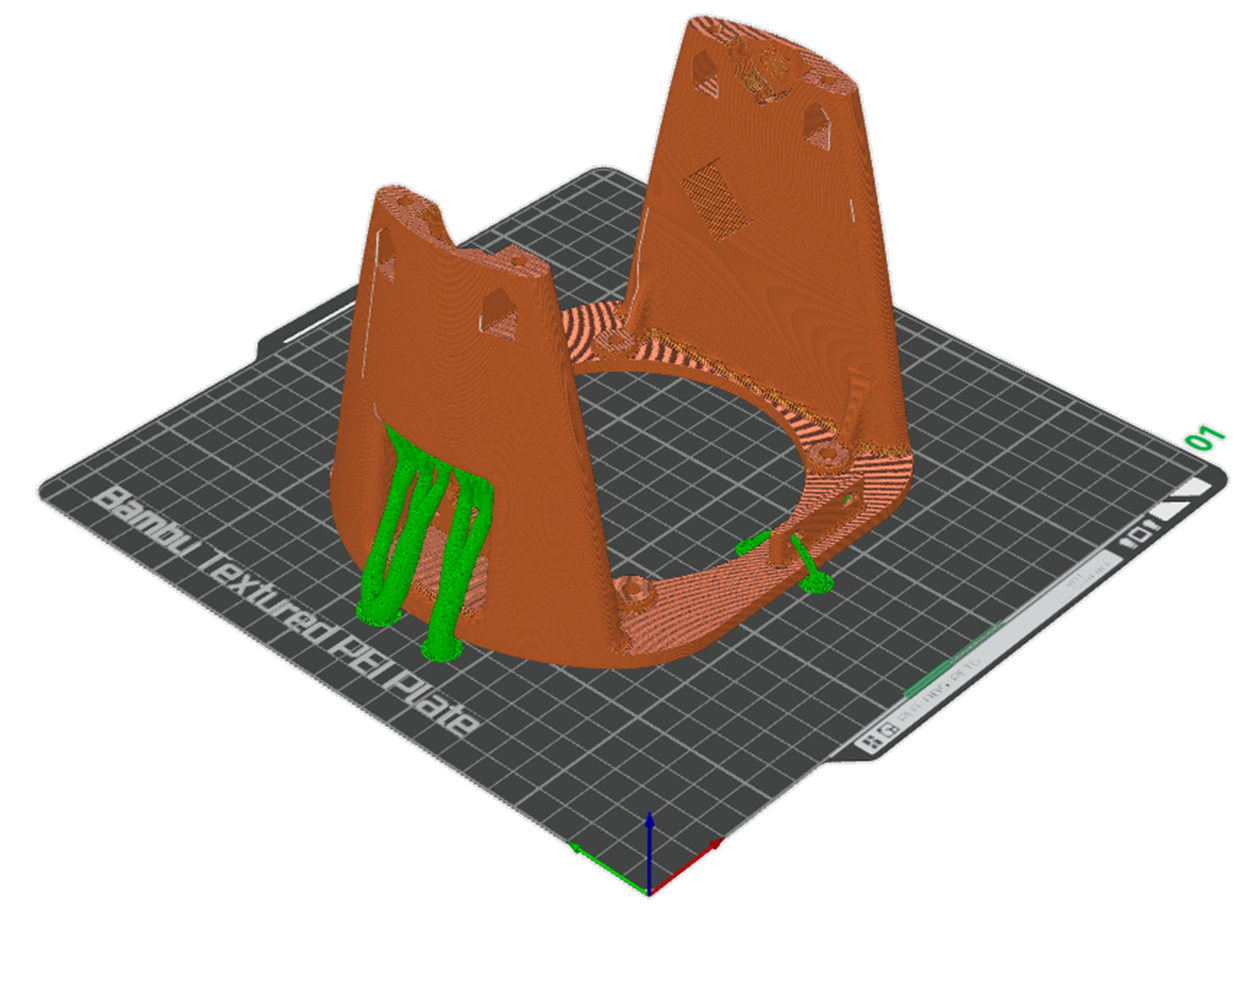
\includegraphics[width=.7\linewidth]{mech_bambustudio1} 
	\caption{Bambu Studio Slicer}
	\label{fig:mech_bambustudio1}
\end{figure}

\pagebreak
\subsection{Összeszerelés}

Ebben a fejezetben leírom az összeszerelés menetét. Először az elektronikát tartó konzollal kezdtem.

\begin{enumerate}
	\item Ráhúztam a motorok tengelyére a kisfogaskerekeket. 
	\item Rácsavaroztam a távtartókat a Raspberry Pi-ra, a Stepper Motor HAT-ra és a DCDC konverterre, majd mind a hármat rácsavaroztam a 3D nyomtatott konzolra. Félretettem az összeállítást.
	\item Összeraktam a torony elemeit, a gearboxot, a tartó elemét és a két végén lévő elemeket. Összecsavaroztam a tervezett furatokon, majd ezt az összeállítást is félretettem. 
	\item Összeállítottam a prototípus 4 lábát és az ezeket tartó hengert. A lábak talpára gumi elemeket ragasztottam, hogy minél stabilabb legyen a rendszer. Félretettem száradni.
	\item Ezután összecsavaroztam a nagy csapágyhoz csatlakozó alkatrészeket, illetve a DT-1000 elemhez rögzítettem az egyik motort. A DT-2000 elemhez ragasztottam a hozzá tartozó fogaskereket.
	\item A prototípus talpát összecsavaroztam az előző pontban lévő elemmel úgy, hogy a keretet is tartsák a csavarok.
	\item A kerethez rögzítettem a megfelelő motort, beragasztottam a relét és a végálláskapcsolókat is. Kábelkötözővel rögzítettem az elektronikai elemek konzolját a kerethez.
	\item A korábban összerakott gearbox összeállítás tengelyeire illesztettem az oda tartozó fogaskereket és a csapágyakat. Így ráhelyeztem a keretre, és a csapágyházak felső felét hozzácsavaroztam a keretre. 
	\item Összeillesztettem a kamera konzolt, és felragasztottam a helyére. Ugyanígy tettem a tárral is. Beillesztettem a lézer modult a helyére.
	\item Összekötöttem a kábeleket, csatlakozókat.
	\item Csatlakoztattam a tápokat és az ethernet-kábelt.
\end{enumerate}
Az elkészült eszközt a \ref{fig:sentry1}. ábrán lehet látni.
\pagebreak

\begin{figure}[h!]
	\centering
	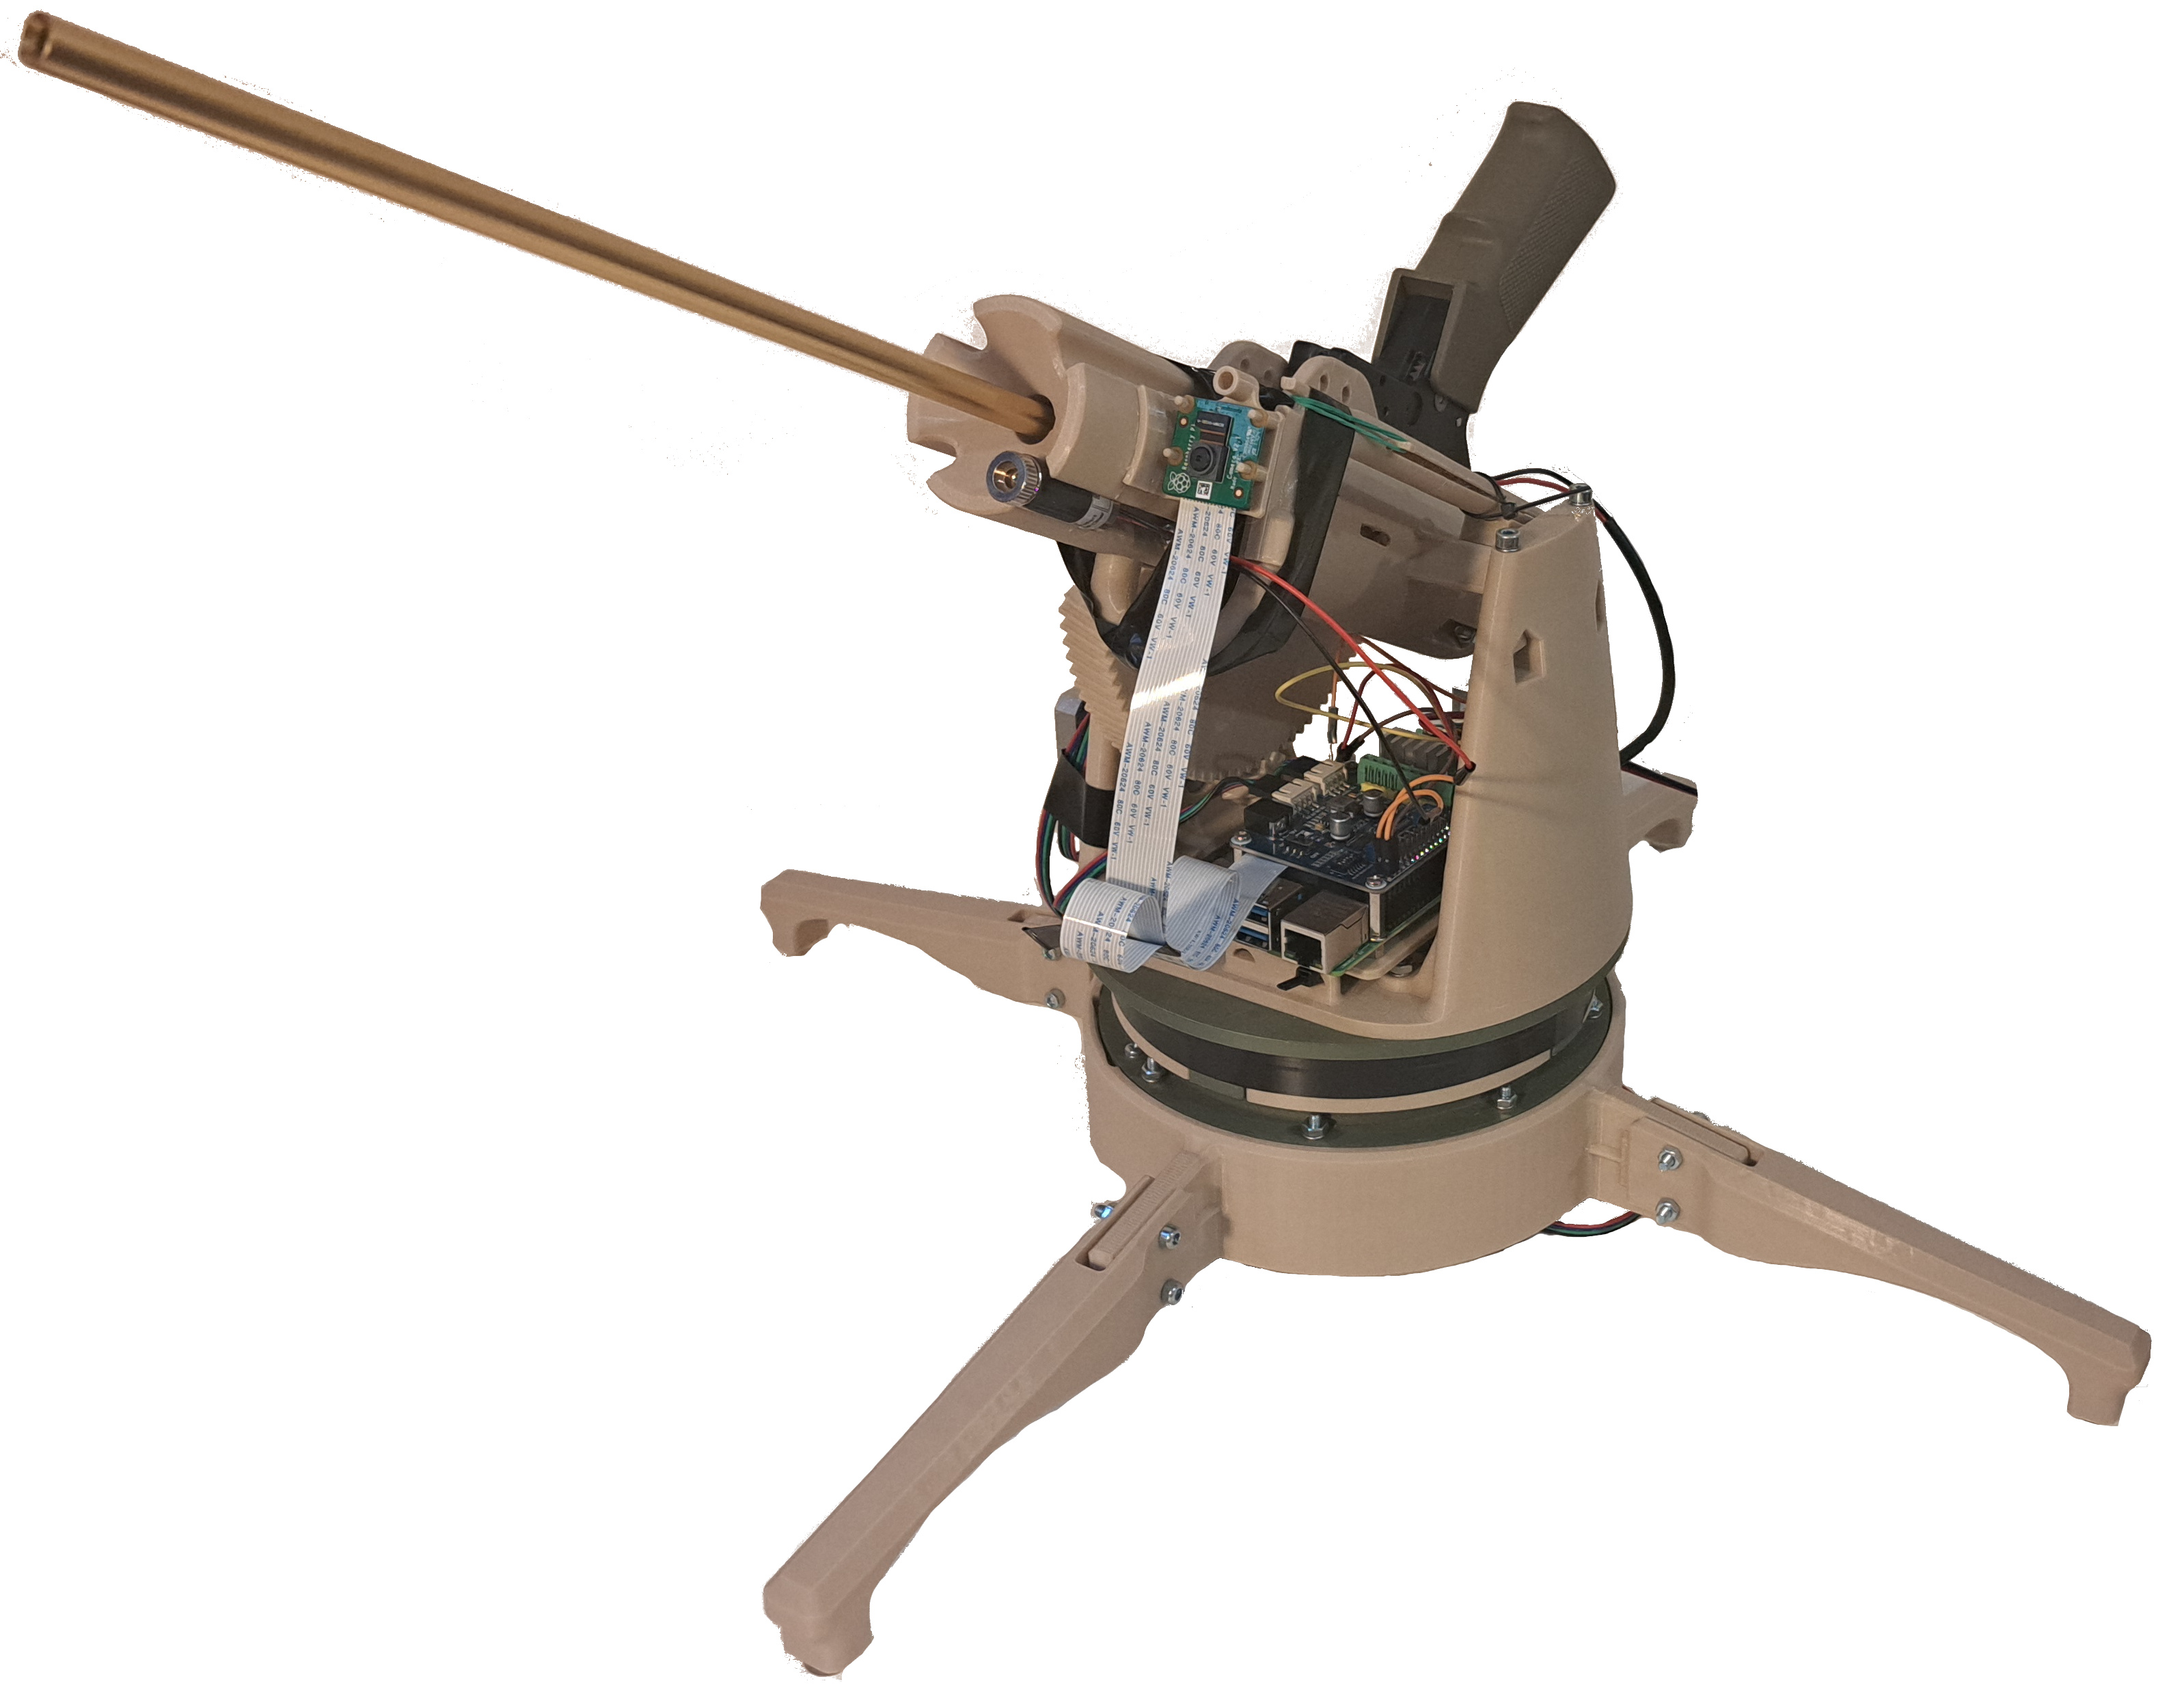
\includegraphics[width=1\linewidth]{sentry1}
	\caption{Összeállított prototípus}
	\label{fig:sentry1}
\end{figure}